\section{Image-to-Image Translation}
The image to image translation model we chose is Cycle Generative Adversarial Network (CycleGAN) developed by Zhu et al~\cite{zhu2017unpaired}.

\subsection{Introduction}
For image-to-image translation task, an original image set $S$ and a target image set $T$ are required. For most of the current I2I models, the two image sets used for training need to be paired, meaning that for every image $s \in S$, there must be a corresponding image $t \in T$. However, this kind of paired image set is scarce because (1) Manual production is time-consuming and laborious (2) The target image set required by some vision and graphics tasks does not exist, such as image translation between painters of different styles. The CycleGAN model proposed by Zhu et al.\ is designed to solve the unpaired image-to-image translation problem. 

The CycleGAN model needs to learn a mapping $G: S \rightarrow T$ between an input image and an output image, which can take the special features of the original image set, and then figure out how to transform these features to the target image set, making it difficult to distinguish between the translated image distribution and the target image set distribution. However, this kind of unpaired unidirectional I2I translation will have an under-constrained problem, that is, the translated image distribution $G(s)$ does match the target image set, but it cannot correspond to the original image $s$ in a meaningful way. This is because there are many mappings $G$ that can generate images with the same distribution. Moreover, this unidirectional training also triggers the well-known problem of mode collapse.

Zhu et al.\ used the property that translation should be ``cycle consistent'' to define another mapping $F: T \rightarrow S$ to reproject the translated image onto the original image, ensuring that $F(G(s))=s$ and $G(F(t))=t$. The model uses two generators and their corresponding discriminators using adversarial loss and defines a novel cycle consistency loss to train the two generators, and discriminators simultaneously. Figure~\ref{figure:cyclegan} shows the basic design of CycleGAN and the Loss definition.

\begin{figure}[!ht]
    \centering
    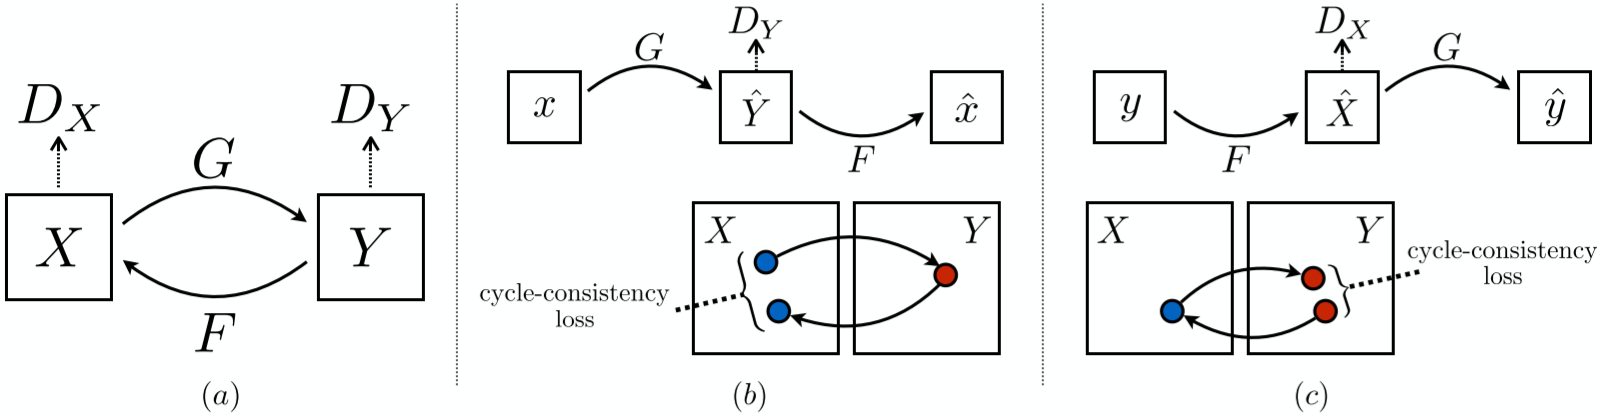
\includegraphics[width=0.9\textwidth]{Section2/cycleGAN.png}
    \caption{(a) The model contains two mapping functions (generators) and associated adversarial discriminators (b) forward cycle-consistency loss (c) backward cycle-consistency loss.}\label{figure:cyclegan}
\end{figure}

\subsection{Model Architecture}
To accomplish I2I, the overall model contains two generators $G: S \rightarrow T$ and $F: T \rightarrow S$ and the corresponding two adversarial discriminators $D_S$ and $D_T$, which are used to distinguish between the original image and the translated image. The basic idea is to improve the accuracy of the adversarial discriminators on image sets $S$ or $T$ while improving the image translation ability of the generators. The ideal result is that the discriminators maintain high accuracy on the image sets $S$ or $T$, but only 50\% accuracy in recognizing the fake images translated by the generators.

\paragraph{Adversarial Loss.}Adversarial loss is applied to generators and discriminators and is mainly used to ensure that the levels of sets of translations from domain S (T) and domain T (S)  are appropriate. Below is the adversarial loss for $G$ and $D_T$. The other one is similar.

\begin{equation}
    \mathcal{L}_{GAN}(G,D_T,S,T) = \mathbb{E}_{t \sim p_{data(t)}}[\log D_T(t)] + \mathbb{E}_{s \sim p_{data(s)}}[\log(1 - D_T(G(s)))]
\end{equation}

\paragraph{Cycle Consistency Loss.} 
To ensure cycle consistency, a reproject error-like forward cycle consistency loss and backward cycle consistency loss, corresponding to two generators respectively, are used, which are defined as:

\begin{equation}
    \mathcal{L}_{cyc}(G,F) = \mathbb{E}_{s \sim p_{data(s)}}[||F(G(s)) - s||_{1}] + \mathbb{E}_{t \sim p_{data(t)}}[||G(F(t)) - t||_{1}]
\end{equation}

Therefore, the full objective function can be defined as:

\begin{equation}
    G^*,F^* = \arg \mathop{\min}_{G,F} \mathop{\max}_{D_S,D_T} \mathcal{L}(G,F,D_T,D_S)
\end{equation}

\begin{equation}
    \mathcal{L}(G,F,D_T,D_S) = \mathcal{L}_{GAN}(G,D_T,S,T) + \mathcal{L}_{GAN}(G,D_S,T,S) + \mathcal{L}_{cyc}(G,F)
\end{equation}

\subsection{Implementation}

\subsubsection{Dataset \& Pre-processing}
What data set do you choose to use

\subsubsection{Discriminator Model}

\subsubsection{Generator Model}

\subsubsection{Training}

\subsection{Result Discussion}
pro cons
\newpage
